%! Author = drakanoy
%! Date = 10.09.2024

% Preamble
\documentclass[12pt]{article}

% Packages
\usepackage[utf8]{inputenc}
\usepackage[T2A]{fontenc}
\usepackage[english, russian]{babel}
\usepackage[a4paper, includefoot, left=1.5cm, right=1.5cm, top=1cm, bottom=1.5cm, headsep=1cm, footskip=1cm]{geometry}
\usepackage{makecell}
\usepackage{amsmath}
\usepackage{graphicx}
\usepackage{enumitem}
\usepackage{svg}
\usepackage{multirow}
\usepackage{hyperref}
\usepackage{mathtools}
\usepackage{amssymb}
\usepackage{textcomp}

% Document
\begin{document}
\begin{large}
\begin{center}
\LARGE \textbf{Домашняя работа}
\par
\LARGE \textbf{Кононов Александр Михайлович}
\par
    \textbf{2.11.2024}
\end{center}
\par Условие:
\par
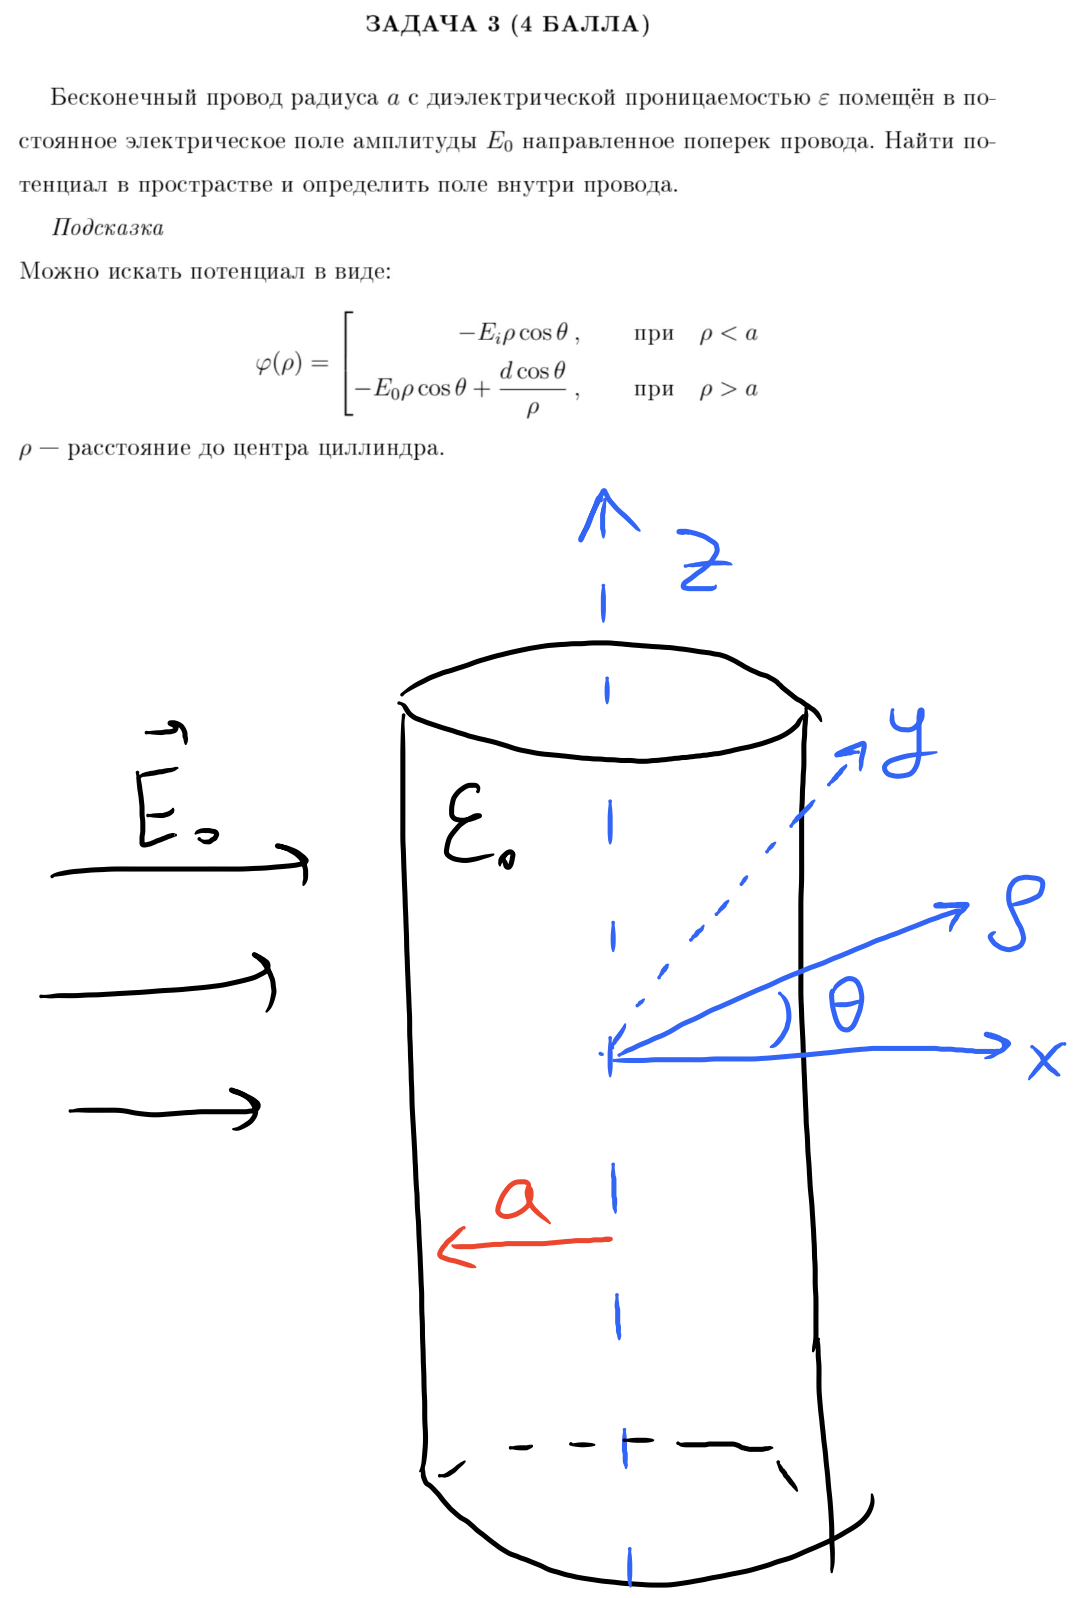
\includegraphics[width=1\textwidth]{photo.png}
%\begin{center}
%\underline{Рисунок 1}:
%\end{center}
\par Решение:
\par
\par
%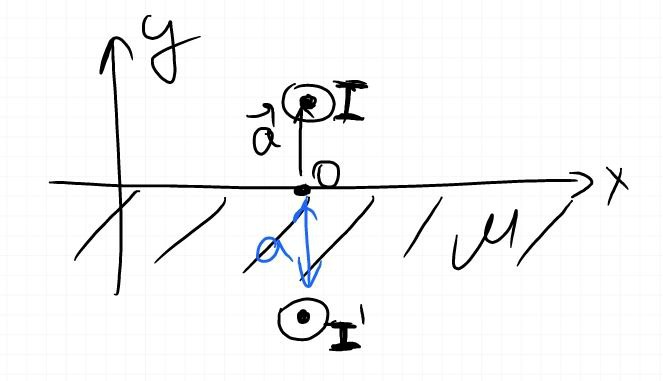
\includegraphics[width=1\textwidth]{photo_1.jpg}
%\par
%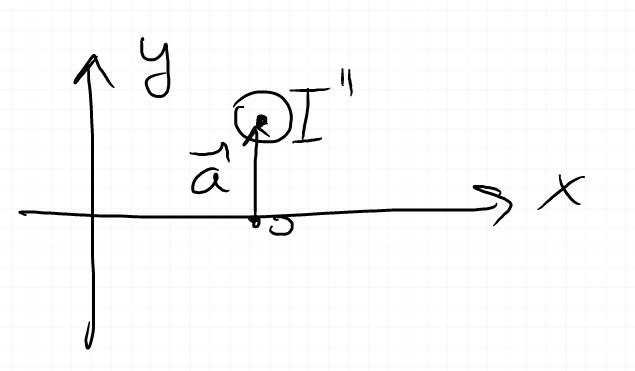
\includegraphics[width=1\textwidth]{photo_2.jpg}
\par
\[
    \xi_3 = \frac{|E_x|^2 - |E_y|^2}{|E_x|^2 + |E_y|^2}
\]
\[
    \xi_1 = \frac{E_x E_y^* + E_y E_x^*}{|E_x|^2 + |E_y|^2}
\]
\[
    \xi_2 = \frac{E_y E_x^* - E_x E_y^*}{i (|E_x|^2 + |E_y|^2)}
\]
\begin{equation*}
    \begin{pmatrix}
        E_{x}^{'} \\
        E_{y}^{'}
    \end{pmatrix}
    =
    \begin{pmatrix}
        \cos \varphi & -\sin \varphi \\
         \sin \varphi & \cos \varphi \\
    \end{pmatrix}
    \cdot
    \begin{pmatrix}
        E_{x} \\
        E_{y}
    \end{pmatrix}
\end{equation*}
\par 1)
\begin{eqnarray*}
%    \nonumber
    |E_{x}^{'}|^2 + |E_{y}^{'}|^2 = |E_{x}|^2 + |E_{y}|^2
\end{eqnarray*}
\par 2)
\begin{eqnarray*}
%    \nonumber
    |E_{x}^{'}|^2 - |E_{y}^{'}|^2 = \left( \cos \varphi \cdot E_x - \sin \varphi \cdot E_y \right)\left( \cos \varphi \cdot E_x^* - \sin \varphi \cdot E_y^* \right) - \\
    - \left( \sin \varphi \cdot E_x + \cos \varphi \cdot E_y \right) \left( \sin \varphi \cdot E_x^* + \cos \varphi \cdot E_y^* \right) = \\
    = \cos^2 \varphi \cdot |E_x|^2 - \cos \varphi \sin \varphi \left( E_x E_y^* + E_y E_x^* \right) + \sin^2 \varphi \cdot |E_y|^2 - \\
    - \left( \sin^2 \varphi \cdot |E_x|^2 + \cos \varphi \sin \varphi \left( E_x E_y^* + E_y E_x^* \right) + \cos^2 \varphi \cdot |E_y|^2 \right) = \\
    = \cos 2 \varphi \left( |E_{x}|^2 - |E_{y}|^2 \right) - \sin 2 \varphi \left( E_x E_y^* + E_y E_x^* \right)
\end{eqnarray*}
\[
    \Rightarrow \xi_3^{'} = \cos 2 \varphi \xi_3 - \sin 2 \varphi \xi_1
\]
\par 3)
\begin{eqnarray*}
%    \nonumber
    E_{x}^{'}E_{y}^{'*} + E_{x}^{'*}E_{y}^{'} = \left( \cos \varphi \cdot E_x - \sin \varphi \cdot E_y \right)\left( \sin \varphi \cdot E_x^* + \cos \varphi \cdot E_y^* \right) + \\
    + \left( \cos \varphi \cdot E_x^* - \sin \varphi \cdot E_y^* \right) \left( \sin \varphi \cdot E_x + \cos \varphi \cdot E_y \right) = \\
    = \cos \varphi \sin \varphi \cdot |E_x|^2 - \cos \varphi \sin \varphi \cdot |E_y|^2 + \cos^2 \varphi \cdot E_x E_y^* - \sin^2 \varphi \cdot E_y E_x^* + \\
    + \cos \varphi \sin \varphi \cdot |E_x|^2 - \cos \varphi \sin \varphi \cdot |E_y|^2 + \cos^2 \varphi \cdot E_x^* E_y - \sin^2 \varphi \cdot E_y^* E_x = \\
    = \sin 2 \varphi \left( |E_{x}|^2 - |E_{y}|^2 \right) + \cos 2 \varphi \left( E_x E_y^* + E_y E_x^* \right)
\end{eqnarray*}
\[
    \Rightarrow \xi_1^{'} = \sin 2 \varphi \xi_3 + \cos 2 \varphi \xi_1
\]
\par 4)
\begin{eqnarray*}
%    \nonumber
    E_{x}^{'*}E_{y}^{'} - E_{x}^{'}E_{y}^{'*} = \left( \cos \varphi \cdot E_x^* - \sin \varphi \cdot E_y^* \right)\left( \sin \varphi \cdot E_x + \cos \varphi \cdot E_y \right) - \\
    - \left( \cos \varphi \cdot E_x - \sin \varphi \cdot E_y \right) \left( \sin \varphi \cdot E_x^* + \cos \varphi \cdot E_y^* \right) = \\
    = \cos \varphi \sin \varphi \cdot |E_x|^2 - \cos \varphi \sin \varphi \cdot |E_y|^2 + \cos^2 \varphi \cdot E_x^* E_y - \sin^2 \varphi \cdot E_y^* E_x - \\
    - \left(  \cos \varphi \sin \varphi \cdot |E_x|^2 - \cos \varphi \sin \varphi \cdot |E_y|^2 + \cos^2 \varphi \cdot E_x E_y^* - \sin^2 \varphi \cdot E_y E_x^*  \right) = \\
    = E_x^* E_y - E_y^* E_x
\end{eqnarray*}
\[
    \Rightarrow \xi_2^{'} = \xi_2
\]
\par Ответ:

\begin{equation*}
    \begin{pmatrix}
        \xi_1^{'} \\
        \xi_2^{'} \\
        \xi_3^{'}
    \end{pmatrix}
    =
    \begin{pmatrix}
        \cos 2 \varphi & 0 & \sin 2 \varphi \\
        0 & 1 & 0 \\
        -\sin 2 \varphi & 0 & \cos 2 \varphi \\
    \end{pmatrix}
    \cdot
    \begin{pmatrix}
        \xi_1 \\
        \xi_2 \\
        \xi_3
    \end{pmatrix}
\end{equation*}

\end{large}
\end{document}
